\documentclass{standalone}

\usepackage{tikz}
\usepackage{pgfplots}

% You may be able to remove this if causing issues
\pgfplotsset{compat=1.11}

\usepackage{helvet}
\renewcommand{\familydefault}{\sfdefault}

\begin{document}

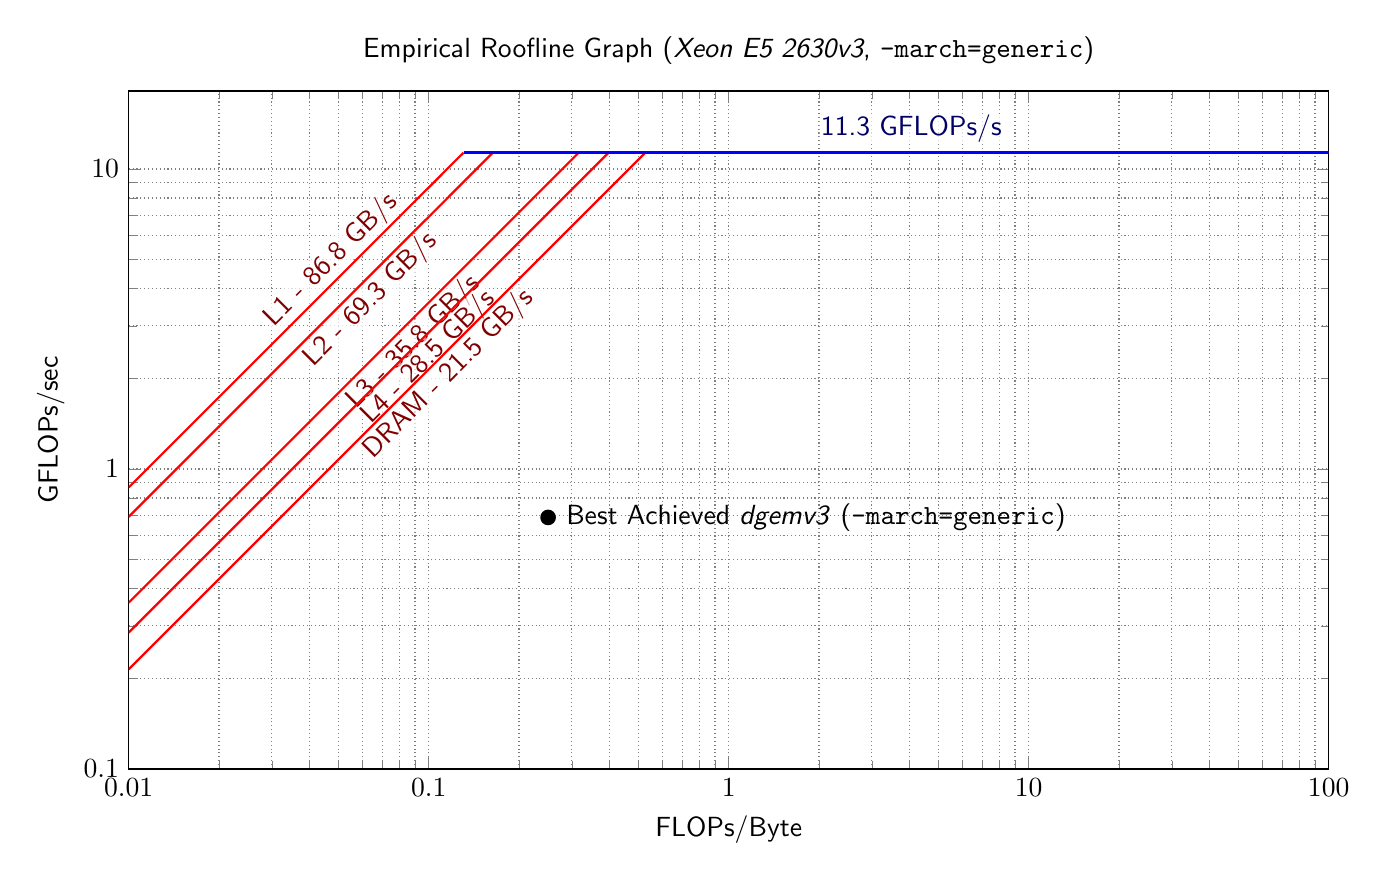
\begin{tikzpicture}
  \pgfplotsset {
    scale only axis,
    axis equal image,
    width=6in,
    /pgf/number format/1000 sep={},
    /tikz/maxline/.style={blue, thick, no marks},
    /tikz/memline/.style={red, thick, no marks},
    /tikz/maxlabel/.style={blue!40!black, right, fill=white, fill opacity=0.7, text opacity=1.0, rounded corners=2pt, inner sep=0.5pt},
    /tikz/memlabel/.style={red!50!black, rotate=45, right, fill=white, fill opacity=0.7, text opacity=1.0, rounded corners=2pt, inner sep=0.5pt}
  }

  \def\Xmin{1.000000e-02}
  \def\Xmax{1.000000e+02}

  \begin{loglogaxis}[
    title={Empirical Roofline Graph (\textit{Xeon E5 2630v3}, \texttt{-march=generic})},
    grid=both,
    grid style={black!50, densely dotted},
    xlabel= FLOPs/Byte,
    ylabel= GFLOPs/sec,
    xmin=\Xmin,
    xmax=\Xmax,
    ymin=1.000000e-01,
    ymax= ,
    log ticks with fixed point
    ]

    \node[maxlabel] at (axis cs: 2.0000000e+00,1.3608000e+01) {11.3 GFLOPs/s};
    \node[memlabel] at (axis cs: 2.8973756e-02,3.0423545e+00) {L1 - 86.8 GB/s};
    \node[memlabel] at (axis cs: 3.9237024e-02,2.2465628e+00) {L2 - 69.3 GB/s};
    \node[memlabel] at (axis cs: 5.4552668e-02,1.6158410e+00) {L3 - 35.8 GB/s};
    \node[memlabel] at (axis cs: 6.1186241e-02,1.4406579e+00) {L4 - 28.5 GB/s};
    \node[memlabel] at (axis cs: 6.2113010e-02,1.1031476e+00) {DRAM - 21.5 GB/s};

    \addplot[memline, domain=(\Xmin:1.3067527e-01)] {8.6780000e+01*x};
    \addplot[memline, domain=(\Xmin:1.6368360e-01)] {6.9280000e+01*x};
    \addplot[memline, domain=(\Xmin:3.1640625e-01)] {3.5840000e+01*x};
    \addplot[memline, domain=(\Xmin:3.9803440e-01)] {2.8490000e+01*x};
    \addplot[memline, domain=(\Xmin:5.2768730e-01)] {2.1490000e+01*x};
    \addplot[maxline, domain=(1.3067527e-01:\Xmax)] {1.1340000e+01};

    \node[label={0:{Best Achieved \textit{dgemv3} (\texttt{-march=generic})}},circle,fill,inner sep=2pt] at (axis cs:0.8/3.2,0.8/1.160198) {};

  \end{loglogaxis}
\end{tikzpicture}

\end{document}
